\documentclass{article}
\usepackage{pstricks}
\usepackage{pst-plot}
\usepackage{graphicx}
\usepackage{son}
\begin{document}
\thispagestyle{empty}

\begin{pspicture}(-4,-3.5)(4,3.5)
%\psgrid[subgriddiv=1,griddots=5,gridlabels=0pt]
%\psset{xunit=1}
%\psset{yunit=1}
%\psline{->}(0,-5)(0,5) % Axe des y
%\psline{->}(-5,0)(5,0) % Axe des x


\rput(-1,1){\resizebox{4cm}{!}{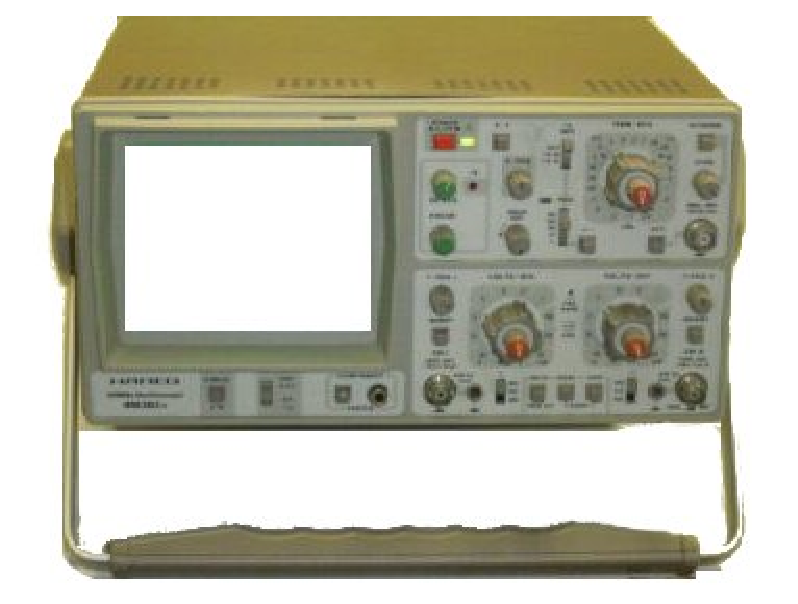
\includegraphics{oscillo.jpg.eps}}}

% signal oscillo


\rput(-3,-2){%
\micro
% fil
\psline{-}(1.4,0)(2.2,0)
\psline{-}(2.2,0)(2.2,2)
\psline{-}(2.2,2)(2,2)
\psline{-}(2.2,2)(2.4,2)
\psline{->}(2,2)(2,2.4)
\psline{->}(2.4,2)(2.4,2.4)
}

\rput(-1.8,1.35){%
\psplot[linecolor=green,linewidth=1pt]{-0.65}{0.65}{x 280 mul 1.2 mul sin 0.45 mul 0.7 mul neg}
}


\end{pspicture}

\end{document}